\section{Modelado y Evaluación de Aprendizaje de Máquina en Spark MLlib}
\label{sec:modelado_evaluacion}

Esta sección desarrolla de forma estructurada los numerales 3, 4, 5 y 6 de la entrega final sobre el clúster de \textbf{Apache Spark} (\texttt{spark://10.195.34.34:7077}) empleando la biblioteca distribuida \textbf{Spark MLlib} (\texttt{pyspark.ml}) \cite{meng2016mllib}, y da respuesta cuantitativa a la \textbf{Pregunta de Negocio 8} sobre las variables asociadas con la fatalidad vial.

\subsection{Selección y Justificación de Técnicas de Aprendizaje de Máquina}
\label{subsec:seleccion_tecnicas_num3}

En correspondencia directa con los objetivos de negocio establecidos en la Sección \ref{sec:entendimiento_negocio}, se seleccionaron una técnica de aprendizaje supervisado y una técnica de aprendizaje no supervisado nativas de \textbf{Spark MLlib}:

\begin{enumerate}
    \item \textbf{Técnica Supervisada --- Regresión Logística Regularizada (\texttt{LogisticRegression}):}
    \begin{itemize}
        \item \textit{Objetivo de negocio asociado (Objetivo 2 --- Vision Zero y Pregunta 8):} Estimar la probabilidad de que una colisión vehicular reportada resulte en al menos una persona fallecida ($\texttt{label} = \mathbb{I}(\texttt{NUMBER OF PERSONS KILLED} > 0) \in \{0, 1\}$) e identificar qué familias de variables (hora, ubicación, tipo de vehículo y factor contribuyente) presentan mayor asociación con un desenlace fatal.
        \item \textit{Justificación técnica y de negocio:} El histórico de colisiones provee una etiqueta binaria verificada para cada siniestro. A diferencia de modelos de caja negra, la Regresión Logística en MLlib permite: (i) incorporar pesos por observación (\texttt{weightCol}) para compensar el desbalance extremo de la clase fatal ($\approx 0.25\%$), (ii) controlar el sobreajuste sobre cientos de categorías codificadas mediante regularización L2 (\texttt{regParam}), y (iii) inspeccionar directamente el signo y la magnitud de los coeficientes ajustados ($\beta_j$), ofreciendo interpretabilidad auditable para las autoridades de transporte y emergencias de Nueva York.
    \end{itemize}

    \item \textbf{Técnica No Supervisada --- Agrupamiento K-Means (\texttt{KMeans}):}
    \begin{itemize}
        \item \textit{Objetivo de negocio asociado (Objetivos 1 y 2 --- Tipología Territorial de Riesgo):} Segmentar las cuadrículas urbanas activas de Nueva York ($0.01^\circ \times 0.01^\circ$) en perfiles homogéneos según su carga conjunta de siniestralidad vial, volumen de arrestos, proporción de accidentes nocturnos y proporción de accidentes con peatones o ciclistas afectados.
        \item \textit{Justificación técnica y de negocio:} Las cuadrículas geográficas carecen de una etiqueta predefinida que las clasifique a priori en tipologías operativas. El algoritmo \texttt{KMeans} distribuido de MLlib particiona el espacio multivariado estandarizado minimizando la suma de distancias euclídeas al cuadrado respecto a los centroides de cada grupo, permitiendo descubrir perfiles territoriales objetivos para diferenciar dónde desplegar estrategias integrales de alta intensidad frente a intervenciones preventivas focalizadas.
    \end{itemize}
\end{enumerate}

\subsection{Preparación de Datos para Modelado}
\label{subsec:prep_modelado_num4}

El proceso de preparación de datos para ambos modelos se estructuró rigurosamente en las tres subetapas exigidas por la metodología:

\subsubsection{Eliminación de Características Fuertemente Correlacionadas}
\label{subsubsec:num4a_correlacion}

Para prevenir problemas de multicolinealidad en la estimación de coeficientes de la Regresión Logística y evitar la redundancia de dimensiones en el cálculo de distancias euclídeas de K-Means, se implementó en PySpark la función distribuida \texttt{seleccionar\_numericas(\allowbreak df, candidatas, limite=0.90)}, la cual ensambla las variables numéricas candidatas mediante \texttt{VectorAssembler}, calcula la matriz de correlación lineal de Pearson en el clúster con \texttt{Correlation.corr(..., 'pearson')} de \texttt{pyspark.ml.stat}, verifica que cada atributo posea desviación estándar poblacional no nula y descarta cualquier variable cuya correlación absoluta con una variable previa supere el umbral $|r| \ge 0.90$.

\paragraph{1. Matriz de correlación para el modelo supervisado (Regresión Logística):}
Calculada sobre el conjunto de entrenamiento (año 2024, $n = 83,698$ colisiones válidas) entre las componentes trigonométricas de la hora (\texttt{hora\_seno}, \texttt{hora\_coseno}) y las coordenadas geográficas (\texttt{lat}, \texttt{lon}). Como muestra la Tabla \ref{tab:corr_lr}, la máxima correlación absoluta es $|r| = 0.35$ (entre latitud y longitud, por la orientación diagonal suroeste--noreste de la geografía de NYC), muy por debajo del umbral de $0.90$, por lo que se conservan las cuatro variables numéricas.

\begin{table}[H]
\centering
\small
\renewcommand{\arraystretch}{1.2}
\caption{Matriz de correlación de Pearson en Spark MLlib para las variables numéricas del modelo supervisado.}
\label{tab:corr_lr}
\begin{tabular}{l r r r r}
\toprule
\textbf{Variable} & \textbf{\texttt{hora\_seno}} & \textbf{\texttt{hora\_coseno}} & \textbf{\texttt{lat}} & \textbf{\texttt{lon}} \\
\midrule
\texttt{hora\_seno} & $1.00$ & $-0.08$ & $0.01$ & $0.02$ \\
\texttt{hora\_coseno} & $-0.08$ & $1.00$ & $0.03$ & $0.04$ \\
\texttt{lat} & $0.01$ & $0.03$ & $1.00$ & $\mathbf{0.35}$ \\
\texttt{lon} & $0.02$ & $0.04$ & $\mathbf{0.35}$ & $1.00$ \\
\bottomrule
\end{tabular}
\end{table}

\paragraph{2. Matriz de correlación para el modelo no supervisado (K-Means):}
Calculada sobre las $699$ cuadrículas urbanas de $0.01^\circ \times 0.01^\circ$ con al menos $10$ colisiones en el primer semestre de 2026. Como se observa en la Tabla \ref{tab:corr_km}, la correlación más alta ocurre entre el volumen logarítmico de colisiones y el de arrestos ($r = 0.78$), reflejando la co-ocurrencia en zonas de alta actividad urbana, pero manteniéndose por debajo del umbral $|r| = 0.90$. En consecuencia, ninguna de las cuatro variables resulta redundante y se conservan todas para el agrupamiento.

\begin{table}[H]
\centering
\scriptsize
\renewcommand{\arraystretch}{1.2}
\caption{Matriz de correlación de Pearson en Spark MLlib para las variables de perfil territorial (K-Means).}
\label{tab:corr_km}
\resizebox{\textwidth}{!}{%
\begin{tabular}{l r r r r}
\toprule
\textbf{Variable} & \textbf{\texttt{log\_colisiones}} & \textbf{\texttt{log\_arrestos}} & \textbf{\texttt{proporcion\_nocturna}} & \textbf{\texttt{proporcion\_vulnerables}} \\
\midrule
\texttt{log\_colisiones} & $1.00$ & $\mathbf{0.78}$ & $0.07$ & $0.35$ \\
\texttt{log\_arrestos} & $\mathbf{0.78}$ & $1.00$ & $-0.02$ & $0.43$ \\
\texttt{proporcion\_nocturna} & $0.07$ & $-0.02$ & $1.00$ & $-0.19$ \\
\texttt{proporcion\_vulnerables} & $0.35$ & $0.43$ & $-0.19$ & $1.00$ \\
\bottomrule
\end{tabular}%
}
\end{table}

\subsubsection{Normalización y Transformación Matemática de Variables Numéricas}
\label{subsubsec:num4b_normalizacion}

Ambos algoritmos seleccionados requieren normalización numérica: en la Regresión Logística con penalización L2 (\texttt{regParam}), las variables continuas deben compartir la misma escala para que la regularización penalice de manera equitativa sus coeficientes; en K-Means, la distancia euclídea al cuadrado es sensible a la magnitud de cada eje, por lo que una variable sin escalar dominaría por completo la asignación de clústeres. Por ello, se aplicaron tres transformaciones matemáticas dentro de los \texttt{Pipeline} de MLlib:

\begin{enumerate}
    \item \textbf{Codificación cíclica de la hora del siniestro:} Dado que la hora entera $h \in \{0, \dots, 23\}$ presenta una discontinuidad artificial en la medianoche ($23:00$ y $00:00$ están a $1$ hora de distancia real pero a $23$ unidades numéricas), se proyectó sobre el círculo unitario mediante:
    \[
    \texttt{hora\_seno} = \sin\!\left(\frac{2\pi \cdot \texttt{hora}}{24}\right), \qquad
    \texttt{hora\_coseno} = \cos\!\left(\frac{2\pi \cdot \texttt{hora}}{24}\right).
    \]
    \item \textbf{Transformación logarítmica estabilizadora en K-Means:} Como los conteos de colisiones y arrestos por cuadrícula presentan fuerte asimetría positiva (colas derechas largas en zonas céntricas), se aplicó la transformación $\texttt{log\_colisiones} = \ln(1 + \texttt{colisiones})$ y $\texttt{log\_arrestos} = \ln(1 + \texttt{arrestos})$ mediante \texttt{F.log1p(...)}.
    \item \textbf{Estandarización Z-score (\texttt{StandardScaler}):} Se aplicó \texttt{StandardScaler(withMean=True, withStd=True)} de \texttt{pyspark.ml.feature}, transformando cada atributo numérico $x_j$ en $z_j = (x_j - \mu_j)/\sigma_j$ con media cero y desviación estándar unitaria. En el modelo supervisado, el \texttt{StandardScaler} y los codificadores categóricos se ajustaron (\texttt{.fit()}) \textbf{exclusivamente sobre el subconjunto de entrenamiento (2024)} y luego se aplicaron (\texttt{.transform()}) sobre validación (2025) y prueba (2026), garantizando cero fuga de información (\textit{data leakage}).
\end{enumerate}

\subsubsection{Selección Final de Variables según Criterio de Negocio}
\label{subsubsec:num4c_seleccion_negocio}

Luego del análisis de correlación del apartado 4.a y la normalización del apartado 4.b, la Tabla \ref{tab:variables_finales_mllib} describe el conjunto definitivo de variables seleccionadas para cada modelo junto con su justificación de negocio.

\begin{table}[H]
\centering
\scriptsize
\renewcommand{\arraystretch}{1.25}
\caption{Grupo final de variables seleccionadas para los modelos supervisado y no supervisado en Spark MLlib.}
\label{tab:variables_finales_mllib}
\begin{tabularx}{\linewidth}{>{\raggedright\arraybackslash}p{2.2cm} >{\raggedright\arraybackslash}p{3.4cm} >{\raggedright\arraybackslash}p{3.0cm} X}
\toprule
\textbf{Modelo} & \textbf{Variable / Familia} & \textbf{Rol y Codificación} & \textbf{Criterio de negocio para su selección o exclusión} \\
\midrule
Reg. Logística & \texttt{label} (Fatalidad) & Objetivo binario $\{0, 1\}$ & Toma el valor $1.0$ si $\texttt{PERSONS KILLED} > 0$ y $0.0$ en caso contrario (prioridad crítica de \textit{Vision Zero}). \\
Reg. Logística & \texttt{hora\_seno}, \texttt{hora\_coseno} & Numéricas escaladas (2 dim.) & Capturan la variación del riesgo letal según la franja horaria (visibilidad nocturna y velocidades de madrugada). \\
Reg. Logística & \texttt{lat}, \texttt{lon} & Numéricas escaladas (2 dim.) & Capturan el gradiente espacial continuo de severidad vial en la red arterial de NYC (\texttt{coord\_valida = True}). \\
Reg. Logística & \texttt{VEHICLE TYPE CODE 1} & Categórica (\texttt{StringIndexer} + \texttt{OneHotEncoder}) & Representa la masa y geometría del vehículo principal involucrado (camiones, SUV, motocicletas, ambulancias, sedanes). \\
Reg. Logística & \texttt{CONTRIBUTING FACTOR 1} & Categórica (\texttt{StringIndexer} + \texttt{OneHotEncoder}) & Representa la causa operativa reportada del siniestro (velocidad, iluminación, distracción, falla mecánica). \\
Reg. Logística & \textit{Excluidas:} \texttt{INJURED} y \texttt{KILLED} & Excluidas de \texttt{features} & \textbf{Exclusión obligatoria por negocio:} Son resultados posteriores al impacto que determinan directamente la etiqueta fatal (\textit{target leakage}). \\
\midrule
K-Means (699) & \texttt{log\_colisiones} & Numérica escalada & Mide el nivel general de exposición y frecuencia de siniestros viales en cada cuadrícula de $0.01^\circ \times 0.01^\circ$. \\
K-Means (699) & \texttt{log\_arrestos} & Numérica escalada & Mide la presión simultánea de criminalidad y demanda policial del NYPD en la misma celda geográfica. \\
K-Means (699) & \texttt{proporcion\_nocturna} & Numérica escalada $[0,1]$ & Fracción de colisiones ocurridas entre las 22:00 y las 05:59 h; orienta operativos de control nocturno e iluminación. \\
K-Means (699) & \texttt{proporcion\_vulnerables} & Numérica escalada $[0,1]$ & Fracción de colisiones con peatones o ciclistas heridos/fallecidos; orienta rediseño peatonal y ciclorrutas de \textit{Vision Zero}. \\
\bottomrule
\end{tabularx}
\end{table}

\subsection{Aplicación de las Técnicas Seleccionadas sobre el Clúster Spark}
\label{subsec:aplicacion_mllib_num5}

\subsubsection{Partición Temporal y Ponderación de Clases en el Modelo Supervisado}

Sobre las colisiones con coordenadas y hora válidas ocurridas entre el 1 de enero de 2024 y el 30 de junio de 2026 ($206,989$ siniestros), se realizó una partición cronológica estricta para simular el despliegue real sobre eventos futuros (Tabla \ref{tab:particion_temporal_lr}).

\begin{table}[H]
\centering
\scriptsize
\renewcommand{\arraystretch}{1.2}
\caption{Partición temporal del conjunto de datos para el modelado supervisado en Spark MLlib.}
\label{tab:particion_temporal_lr}
\resizebox{\textwidth}{!}{%
\begin{tabular}{l c r r r r}
\toprule
\textbf{Subconjunto} & \textbf{Periodo} & \textbf{No fatales (\texttt{0.0})} & \textbf{Fatales (\texttt{1.0})} & \textbf{Total colisiones} & \textbf{Prevalencia fatal} \\
\midrule
Entrenamiento (\texttt{train\_lr}) & Año 2024 & 83,479 & 219 & 83,698 & 0.2617\% \\
Validación (\texttt{val\_lr}) & Año 2025 & 82,713 & 205 & 82,918 & 0.2472\% \\
Prueba (\texttt{test\_lr}) & 2026-I (Ene--Jun) & 40,271 & 102 & 40,373 & 0.2526\% \\
\bottomrule
\end{tabular}%
}
\end{table}

El pipeline de preparación (\texttt{VectorAssembler} $\rightarrow$ \texttt{StandardScaler} $\rightarrow$ \texttt{StringIndexer(handleInvalid='keep')} $\rightarrow$ \texttt{OneHotEncoder} $\rightarrow$ \texttt{VectorAssembler}) generó un vector disperso de \textbf{$347$ características} (\texttt{features}). Dado que en el entrenamiento solo existen $219$ colisiones fatales frente a $83,479$ no fatales, un clasificador sin ponderación predeciría siempre la clase mayoritaria. Para corregirlo, se asignó a cada registro fatal del conjunto de entrenamiento un peso inversamente proporcional a su frecuencia:
\[
w_i = \begin{cases}
\dfrac{N_{0,\text{train}}}{N_{1,\text{train}}} = \dfrac{83{,}479}{219} \approx 381.18, & \text{si } \texttt{label}_i = 1.0, \\[8pt]
1.0, & \text{si } \texttt{label}_i = 0.0,
\end{cases}
\]
pasando la columna \texttt{peso} al parámetro \texttt{weightCol='peso'} de \texttt{LogisticRegression} en MLlib, mientras que los conjuntos de validación y prueba se evaluaron con su distribución real sin alterar.

\subsection{Evaluación de los Modelos de Aprendizaje de Máquina}
\label{subsec:evaluacion_modelos_num6}

\subsubsection{Evaluación Paramétrica del Modelo Supervisado (Regresión Logística)}

Dado el fuerte desbalance de clases ($\text{prevalencia} = 0.0025$), la exactitud global (\textit{accuracy}) no es una métrica adecuada (un modelo trivial que prediga siempre \texttt{0} tendría $99.75\%$ de exactitud y $0\%$ de utilidad para \textit{Vision Zero}). Por ello, se seleccionaron como métricas principales el \textbf{Área Bajo la Curva Precisión--Recall (AUPRC)}, cuya línea base de azar es la prevalencia de la clase positiva ($0.0025$), el \textbf{Área Bajo la Curva ROC (AUROC)} y, para la toma de decisiones binaria, la \textbf{Precisión}, la \textbf{Exhaustividad (\textit{Recall})} y la media armónica \textbf{F1}.

\paragraph{1. Búsqueda del parámetro de regularización (\texttt{regParam}):}
Se entrenaron tres modelos en el clúster variando $\texttt{regParam} \in \{0.01, 0.10, 1.00\}$ con $\texttt{maxIter} = 50$ y se evaluaron sobre el conjunto de validación (2025). Como muestra la Tabla \ref{tab:lr_regparam}, una regularización más fuerte ($\texttt{regParam} = 1.00$) obtuvo la mayor AUPRC en validación ($0.004822$, casi el doble de la prevalencia base de $0.002472$), al evitar el sobreajuste de los coeficientes sobre categorías vehiculares o causales poco frecuentes.

\begin{table}[H]
\centering
\small
\renewcommand{\arraystretch}{1.2}
\caption{Evaluación del hiperparámetro de regularización (\texttt{regParam}) de la Regresión Logística en validación (2025).}
\label{tab:lr_regparam}
\begin{tabular}{c c r}
\toprule
\textbf{Parámetro \texttt{regParam}} & \textbf{Iteraciones máximas (\texttt{maxIter})} & \textbf{AUPRC en Validación (2025)} \\
\midrule
$0.01$ & $50$ & $0.004247$ \\
$0.10$ & $50$ & $0.004604$ \\
$\mathbf{1.00}$ & $\mathbf{50}$ & $\mathbf{0.004822}$ \\
\bottomrule
\end{tabular}
\end{table}

\paragraph{2. Calibración del umbral de decisión ($\tau$) en validación:}
Con el modelo óptimo ($\texttt{regParam} = 1.00$), se evaluaron siete umbrales de probabilidad $\tau \in \{0.10, 0.25, 0.40, 0.55, 0.70, 0.85, 0.95\}$ sobre validación (Tabla \ref{tab:lr_umbrales_val}). El umbral $\tau = 0.55$ maximizó el puntaje F1 en validación ($\text{F1} = 0.0071$, con exhaustividad del $47.80\%$ y precisión del $0.36\%$).

\begin{table}[H]
\centering
\small
\renewcommand{\arraystretch}{1.2}
\caption{Evaluación de umbrales de clasificación ($\tau$) para la Regresión Logística ($\texttt{regParam}=1.00$) en validación (2025).}
\label{tab:lr_umbrales_val}
\begin{tabular}{c r r r r r r r}
\toprule
\textbf{Umbral ($\tau$)} & \textbf{VP} & \textbf{FP} & \textbf{FN} & \textbf{VN} & \textbf{Precisión} & \textbf{Exhaustividad (\textit{Recall})} & \textbf{Puntaje F1} \\
\midrule
$0.10$ & 205 & 82,713 & 0 & 0 & $0.0025$ & $1.0000$ & $0.0049$ \\
$0.25$ & 205 & 82,713 & 0 & 0 & $0.0025$ & $1.0000$ & $0.0049$ \\
$0.40$ & 201 & 76,490 & 4 & 6,223 & $0.0026$ & $0.9805$ & $0.0052$ \\
$\mathbf{0.55}$ & $\mathbf{98}$ & $\mathbf{27,394}$ & $\mathbf{107}$ & $\mathbf{55,319}$ & $\mathbf{0.0036}$ & $\mathbf{0.4780}$ & $\mathbf{0.0071}$ \\
$0.70$ & 0 & 20 & 205 & 82,693 & $0.0000$ & $0.0000$ & $0.0000$ \\
$0.85$ & 0 & 0 & 205 & 82,713 & $0.0000$ & $0.0000$ & $0.0000$ \\
$0.95$ & 0 & 0 & 205 & 82,713 & $0.0000$ & $0.0000$ & $0.0000$ \\
\bottomrule
\end{tabular}
\end{table}

\paragraph{3. Desempeño final en el conjunto de prueba independiente (2026-I):}
Al aplicar el modelo elegido ($\texttt{regParam} = 1.00, \tau = 0.55$) sobre las $40,373$ colisiones del primer semestre de 2026 (Tabla \ref{tab:lr_test_final}), se obtuvo una \textbf{$\text{AUPRC} = 0.0042$} ( un $68\%$ por encima de la prevalencia base de $0.0025$) y una \textbf{$\text{AUROC} = 0.5397$}. El clasificador detectó \textbf{$50$ de las $102$ colisiones fatales reales} ($\text{exhaustividad} = 49.02\%$), dejando $52$ sin detectar y generando $16,382$ falsos positivos ($\text{precisión} = 0.30\%$, $\text{F1} = 0.0060$).

\begin{table}[H]
\centering
\small
\renewcommand{\arraystretch}{1.2}
\caption{Desempeño de la Regresión Logística en el conjunto de prueba temporal (primer semestre de 2026).}
\label{tab:lr_test_final}
\begin{tabular}{c c c c r r r r r r r}
\toprule
\textbf{regParam} & \textbf{Umbral} & \textbf{AUPRC} & \textbf{AUROC} & \textbf{VP} & \textbf{FP} & \textbf{FN} & \textbf{VN} & \textbf{Precisión} & \textbf{Recall} & \textbf{F1} \\
\midrule
$1.00$ & $0.55$ & $0.0042$ & $0.5397$ & 50 & 16,382 & 52 & 23,889 & $0.0030$ & $0.4902$ & $0.0060$ \\
\bottomrule
\end{tabular}
\end{table}

\paragraph{4. Respuesta a la Pregunta 8 --- Importancia relativa de variables por familia:}
La Tabla \ref{tab:q8_coeficientes} y la Figura \ref{fig:q8_coeficientes} presentan el predictor con mayor magnitud de coeficiente absoluto ($|\beta_j|$) dentro de cada una de las cuatro familias de variables del modelo ajustado.

\begin{table}[H]
\centering
\small
\renewcommand{\arraystretch}{1.2}
\caption{Mayor coeficiente en magnitud absoluta por familia de variables en la Regresión Logística ajustada (Pregunta 8).}
\label{tab:q8_coeficientes}
\begin{tabular}{l l r r}
\toprule
\textbf{Familia de Variables} & \textbf{Atributo codificado representativo} & \textbf{Coeficiente ($\beta_j$)} & \textbf{Magnitud ($|\beta_j|$)} \\
\midrule
Tipo de vehículo 1 & \texttt{vehiculo\_ohe\_AMBULANE} & $-0.5000$ & $\mathbf{0.5000}$ \\
Factor contribuyente 1 & \texttt{factor\_ohe\_OTHER LIGHTING DEFECTS} & $+0.4098$ & $\mathbf{0.4098}$ \\
Hora del siniestro & \texttt{hora\_coseno} & $+0.0752$ & $0.0752$ \\
Coordenadas geográficas & \texttt{lat} (Latitud estandarizada) & $+0.0070$ & $0.0070$ \\
\bottomrule
\end{tabular}
\end{table}

\begin{figure}[H]
    \centering
    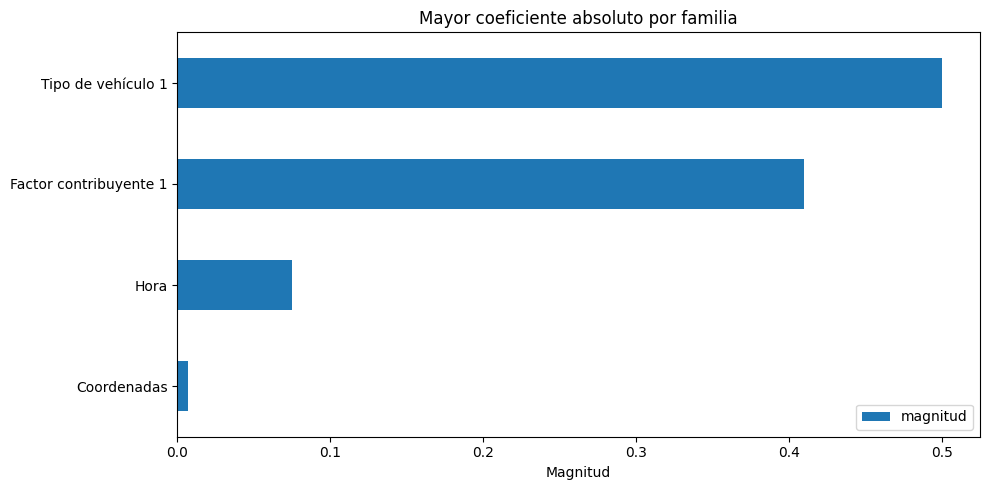
\includegraphics[width=0.82\textwidth]{imagenes/fig_cell_71_1.png}
    \caption{Comparación de la mayor magnitud absoluta de coeficiente ($|\beta_j|$) por familia de variables en la Regresión Logística.}
    \label{fig:q8_coeficientes}
\end{figure}

\noindent \textbf{Interpretación para la Pregunta 8 y punto de contacto con el negocio:}
Las familias categóricas de \textbf{Tipo de vehículo 1 ($|\beta|_{\max} = 0.5000$)} y \textbf{Factor contribuyente 1 ($|\beta|_{\max} = 0.4098$)} concentran el mayor peso discriminativo del modelo lineal, seguidas por la componente nocturna de la hora (\texttt{hora\_coseno}, $+0.0752$, que toma sus valores máximos positivos en las horas cercanas a la medianoche y la madrugada) y las coordenadas continuas (\texttt{lat}, $+0.0070$). Por ejemplo, defectos de iluminación (\texttt{OTHER LIGHTING DEFECTS}, $\beta = +0.4098$) incrementan el puntaje de riesgo fatal, mientras que colisiones de unidades de emergencia (\texttt{AMBULANE}, $\beta = -0.5000$) suelen reportarse incluso en incidentes de baja energía cinética por protocolo administrativo. Al mismo tiempo, la modesta capacidad predictiva global del modelo lineal ($\text{AUROC} = 0.5397$) demuestra dos realidades críticas para los tomadores de decisiones: (i) una combinación puramente lineal no captura las interacciones cruzadas entre hora, zona y vehículo (lo que motiva la implementación de la Red Neuronal Profunda en la Sección \ref{sec:bono_dl}, que eleva el AUROC a $0.6020$), y (ii) el formulario policial MV-104AN carece de variables cinemáticas directas como la velocidad estimada de impacto, el uso de cinturón/casco o el ancho de la vía.

\subsubsection{Evaluación Paramétrica del Modelo No Supervisado (K-Means)}

Sobre las $699$ cuadrículas urbanas activas ($\ge 10$ colisiones en el primer semestre de 2026) estandarizadas con \texttt{StandardScaler}, se ejecutó el algoritmo \texttt{KMeans} de MLlib (\texttt{seed=42}) probando tres valores del hiperparámetro $k \in \{2, 3, 4\}$ y evaluando la cohesión y separación de los grupos mediante el \textbf{coeficiente de Silhouette} con medida de distancia euclídea al cuadrado (\texttt{ClusteringEvaluator}).

\begin{table}[H]
\centering
\small
\renewcommand{\arraystretch}{1.2}
\caption{Evaluación del hiperparámetro $k$ en K-Means mediante el coeficiente de Silhouette en Spark MLlib.}
\label{tab:kmeans_silhouette}
\begin{tabular}{c c r}
\toprule
\textbf{Número de clústeres ($k$)} & \textbf{Medida de distancia} & \textbf{Coeficiente de Silhouette} \\
\midrule
$\mathbf{2}$ & \textbf{Euclídea al cuadrado (\texttt{squaredEuclidean})} & $\mathbf{0.473409}$ \\
$3$ & Euclídea al cuadrado (\texttt{squaredEuclidean}) & $0.459737$ \\
$4$ & Euclídea al cuadrado (\texttt{squaredEuclidean}) & $0.369069$ \\
\bottomrule
\end{tabular}
\end{table}

La configuración óptima corresponde a \textbf{$k = 2$ grupos ($\text{Silhouette} = 0.4734$)}, seguida de cerca por $k = 3$ ($0.4597$), mientras que $k = 4$ fragmenta excesivamente el espacio ($0.3691$). La Tabla \ref{tab:kmeans_perfiles} presenta los promedios de cada grupo reexpresados en sus unidades originales de negocio, y la Figura \ref{fig:kmeans_mapa} muestra su distribución geográfica sobre el mapa de Nueva York.

\begin{table}[H]
\centering
\scriptsize
\renewcommand{\arraystretch}{1.25}
\caption{Caracterización de los perfiles territoriales identificados por K-Means ($k=2$) en unidades originales (2026-I).}
\label{tab:kmeans_perfiles}
\setlength{\tabcolsep}{4pt}
\begin{tabularx}{\linewidth}{l c r r r r r X}
\toprule
\textbf{Clúster} & \textbf{Zonas} & \textbf{Colis.} & \textbf{Arrestos} & \textbf{Fatales} & \textbf{Noct.} & \textbf{Vuln.} & \textbf{Perfil territorial de negocio} \\
\midrule
\textbf{Grupo 0} & 351 & \textbf{83.815} & \textbf{365.991} & \textbf{0.171} & 20.3\% & \textbf{17.3\%} & \textbf{Zonas críticas de alta densidad e interacción vulnerable} (corredores centrales de Manhattan, Brooklyn, Bronx y ejes de Queens). \\
\textbf{Grupo 1} & 348 & 29.296 & 35.330 & 0.101 & 21.0\% & 8.7\% & \textbf{Zonas periféricas y residenciales de baja carga dual} (Staten Island, este de Queens y bordes costeros). \\
\bottomrule
\end{tabularx}
\end{table}

\begin{figure}[H]
    \centering
    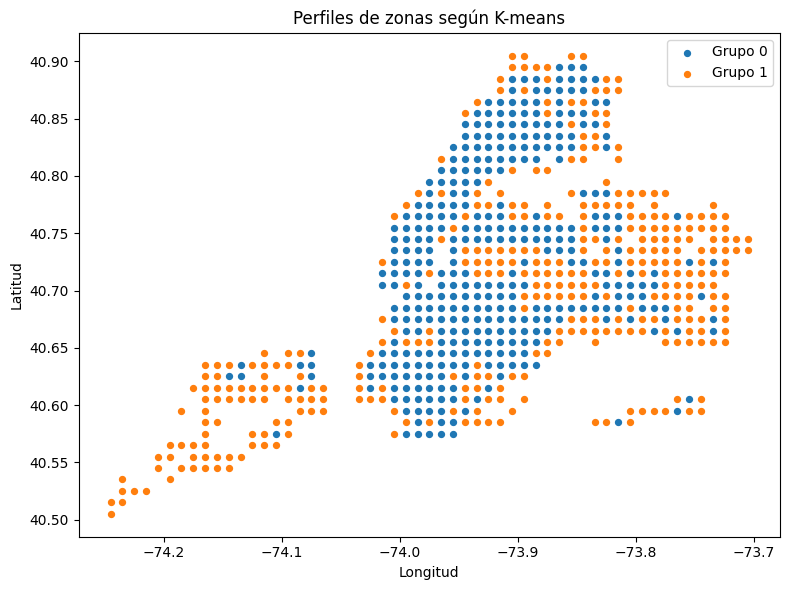
\includegraphics[width=0.76\textwidth]{imagenes/fig_cell_74_1.png}
    \caption{Distribución espacial de las 699 cuadrículas urbanas de Nueva York según los perfiles territoriales del modelo K-Means ($k=2$).}
    \label{fig:kmeans_mapa}
\end{figure}

\noindent \textbf{Interpretación de los perfiles K-Means para la toma de decisiones:}
El agrupamiento divide casi en dos mitades exactas las cuadrículas activas de la ciudad, pero con una asimetría operativa dramática:
\begin{itemize}
    \item \textbf{Grupo 0 ($351$ zonas --- Prioridad Operativa Alta):} Promedia \textbf{$83.8$ colisiones y $366.0$ arrestos por cuadrícula} (más de $10$ veces el volumen de arrestos del Grupo 1 y casi $3$ veces su volumen de colisiones), registra un $69\%$ más de colisiones fatales promedio ($0.171$ vs. $0.101$) y \textbf{duplica exactamente la proporción de choques con peatones o ciclistas heridos o fallecidos ($17.3\%$ frente a $8.7\%$)}. Espacialmente (Figura \ref{fig:kmeans_mapa}, puntos azules), conforma un corredor continuo que abarca Manhattan, el oeste y centro de Brooklyn, el sur y centro del Bronx y el eje central de Queens.
    \item \textbf{Grupo 1 ($348$ zonas --- Prioridad Preventiva y Vial Suburbana):} Promedia $29.3$ colisiones y $35.3$ arrestos por zona, con baja proporción de peatones/ciclistas afectados ($8.7\%$) pero una proporción de siniestralidad nocturna ligeramente superior ($21.0\%$ vs. $20.3\%$). Espacialmente (puntos naranjas), cubre Staten Island, el oriente de Queens y sectores periféricos de Brooklyn y el Bronx, donde predominan desplazamientos en automóvil particular y autopistas periféricas.
\end{itemize}
